%Chapter 4 gets to implementation. Explain each pipeline algorithm in sequence
\chapter{Implementation}
\label{chap:implementation}
This chapter will explore in great detail the functionality and implementation of this thesis's pipeline. As a reminder, the pipeline consists of the highlighted elements in Figure~\ref{fig:toplevelpipeline}. Each section of this chapter describes the implementation of one of these functional blocks.

\section{RGB-D Framework Library}
A crucial component of the pipeline is being able to easily collect RGB-D sensor data from a variety of sources in such a way that the origin of the data is hidden from the remainder of the pipeline. To that end, a highly modular and easily extensible framework library was built to seamlessly convert the native data formats and streaming behavior of different 
\begin{figure}[ht]
    \centering
    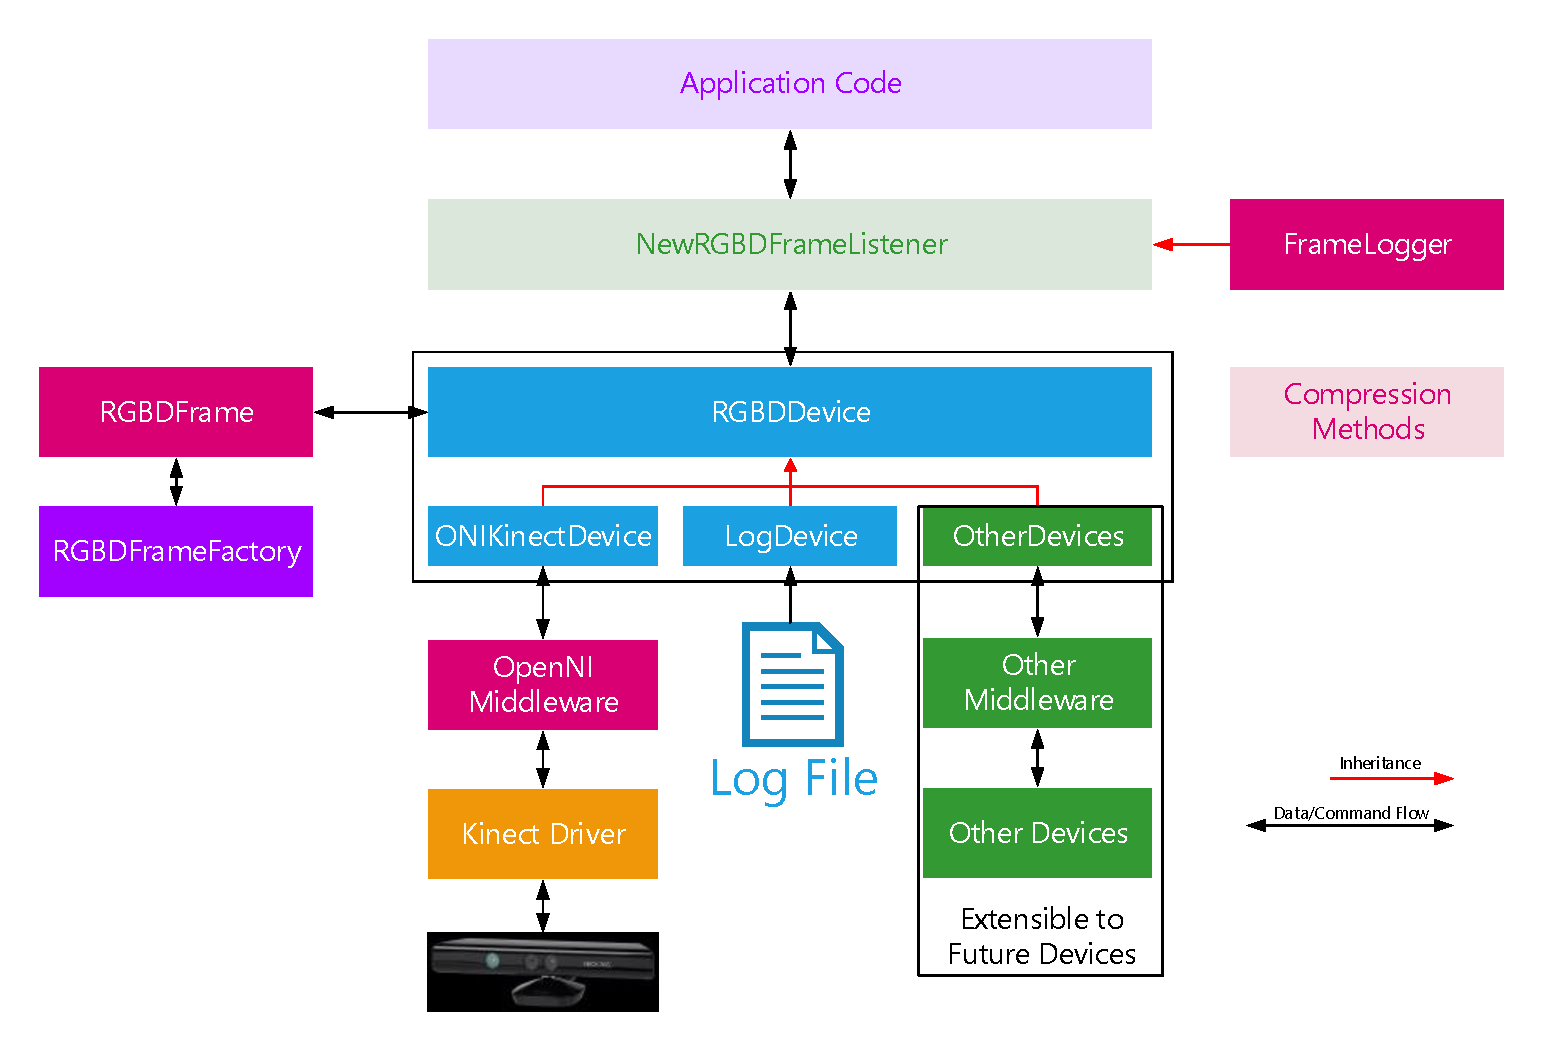
\includegraphics[width=1.0\textwidth]{FrameworkLayout.pdf}
    \caption{RGB-D framework architecture}
    \label{fig:rgbdframework}
\end{figure}

\section{Preprocessing: Filtering and Point Cloud Generation}

\section{Plane Segmentation}
\section{Planar Mesh Generation}